\section{Small stereo roads}
\label{sec:stereoroads}

Proposal and performance of small stereo roads.

\begin{figure}[!htpb]
  \begin{center}
    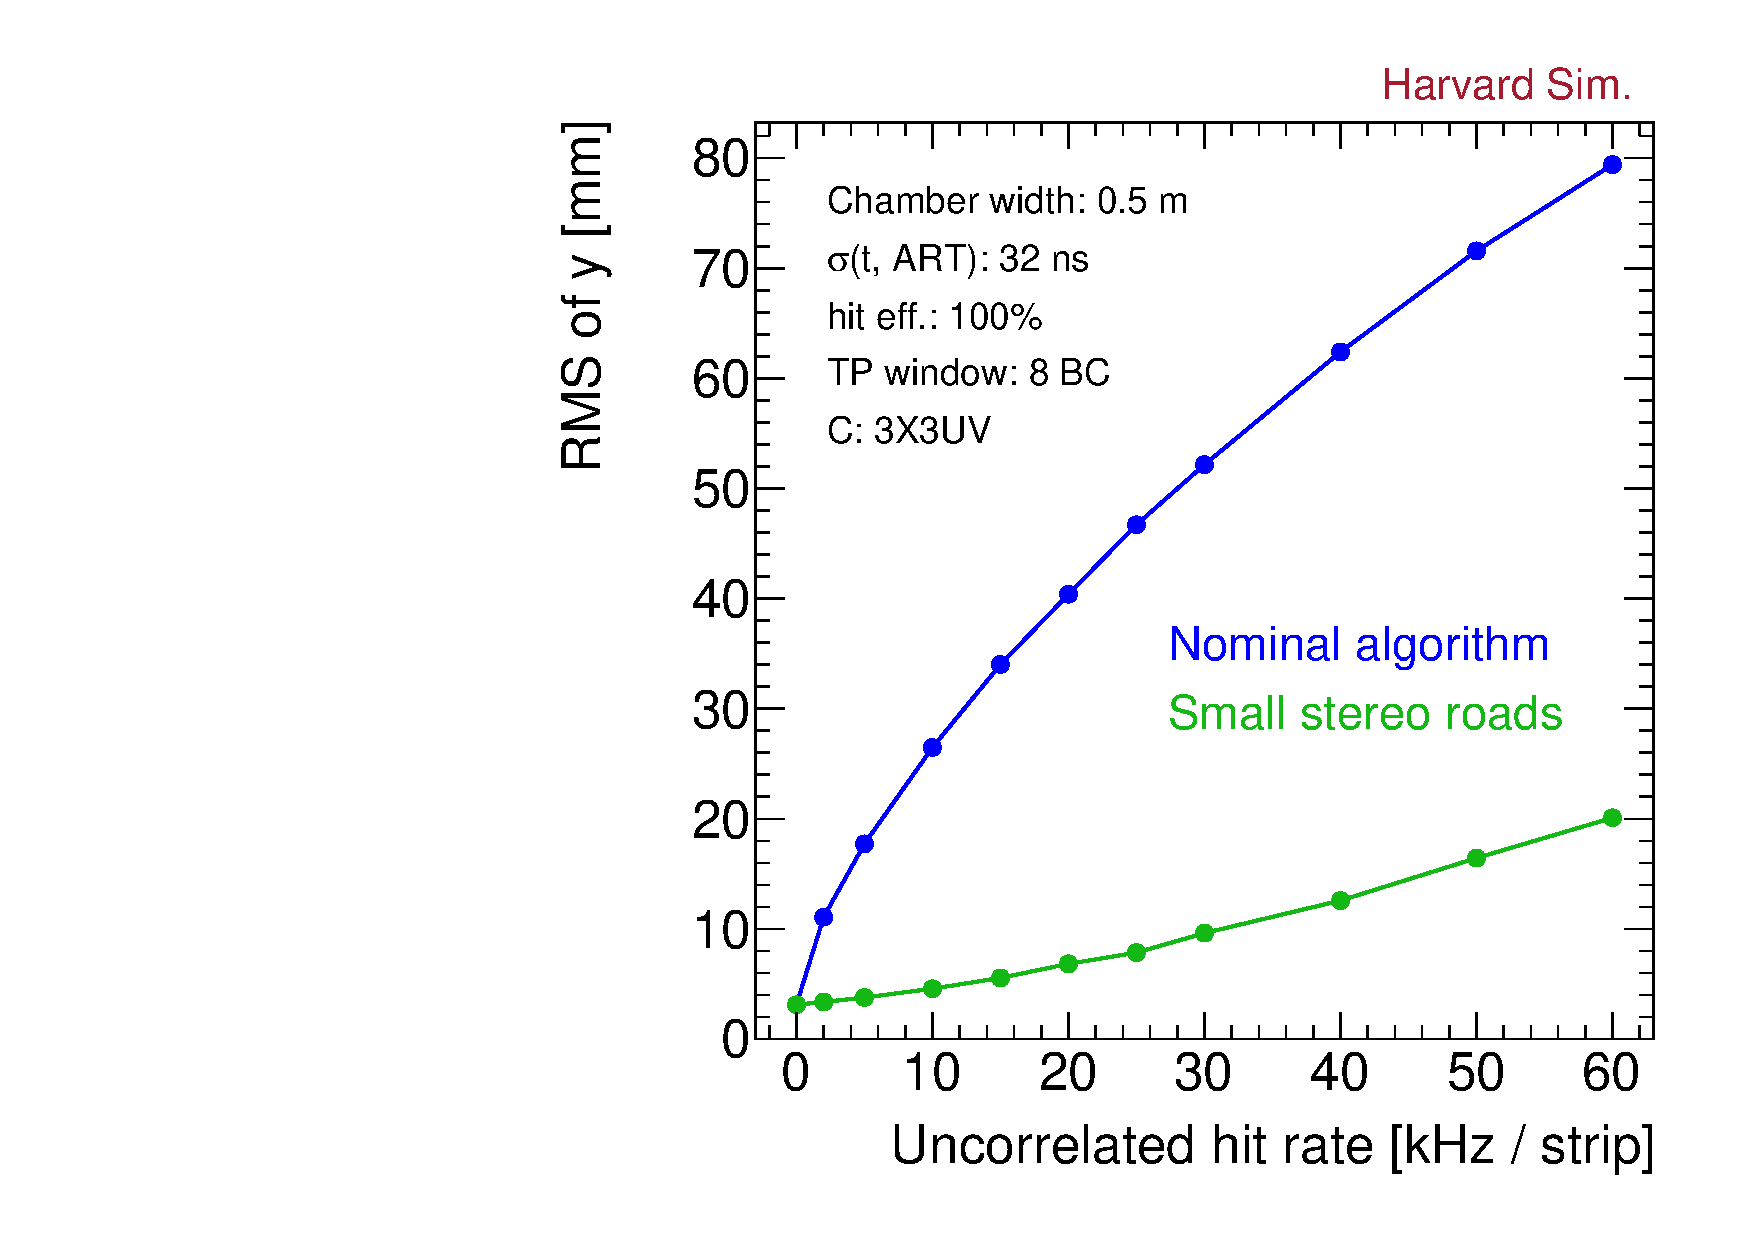
\includegraphics[width=0.48\textwidth]{figures/rms_y_small_vs_rate.pdf}
    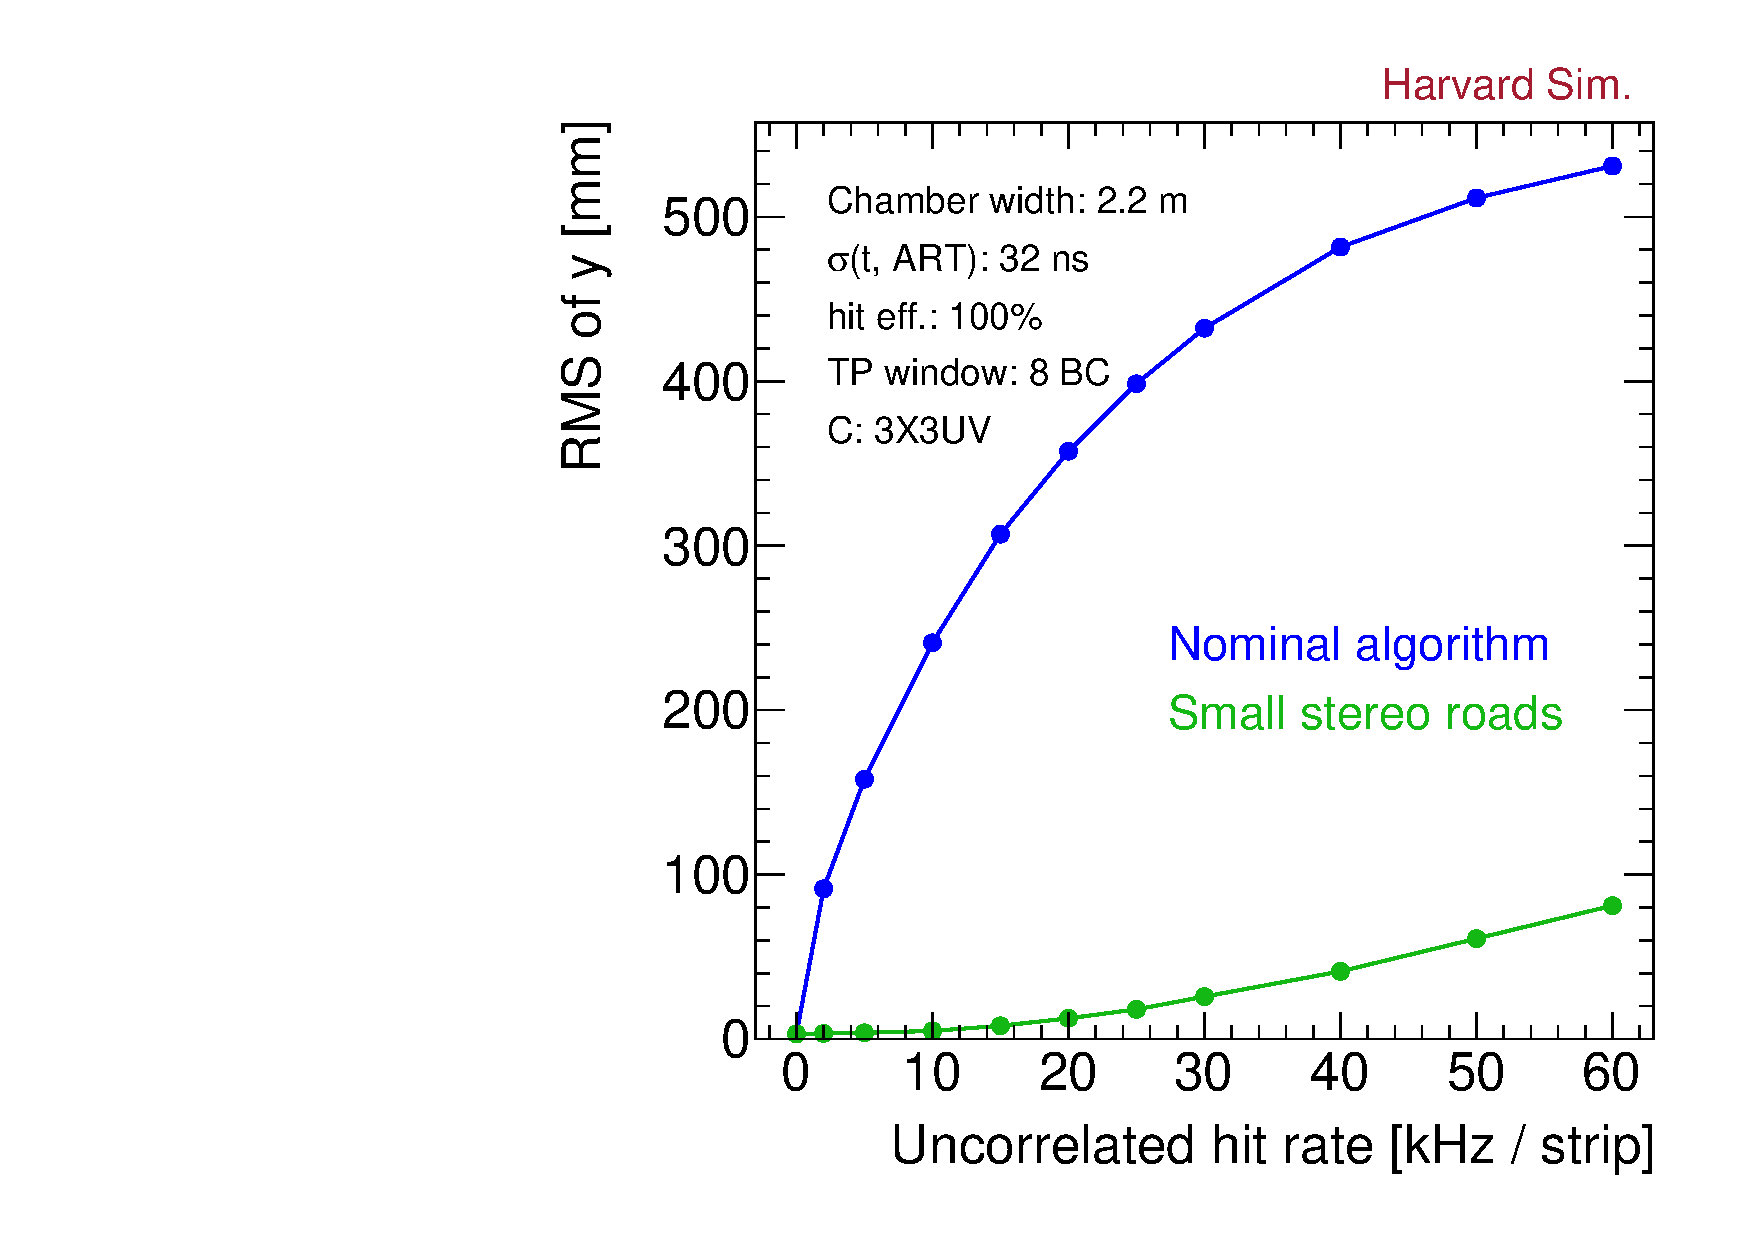
\includegraphics[width=0.48\textwidth]{figures/rms_y_large_vs_rate.pdf}
  \end{center}
  \vspace{-10pt}
  \caption{RMS of $y_\text{reco.} - y_\text{truth}$ for a small chamber of width 0.5m (left) and large chamber of width 2.2m (right) as a function of uncorrelated background rate. The RMS is calculated in the $3\sigma$ (99.7\%) range of the distribution.}
  \label{fig:rms_vs_rate}
\end{figure}

\begin{figure}[!htpb]
  \begin{center}
    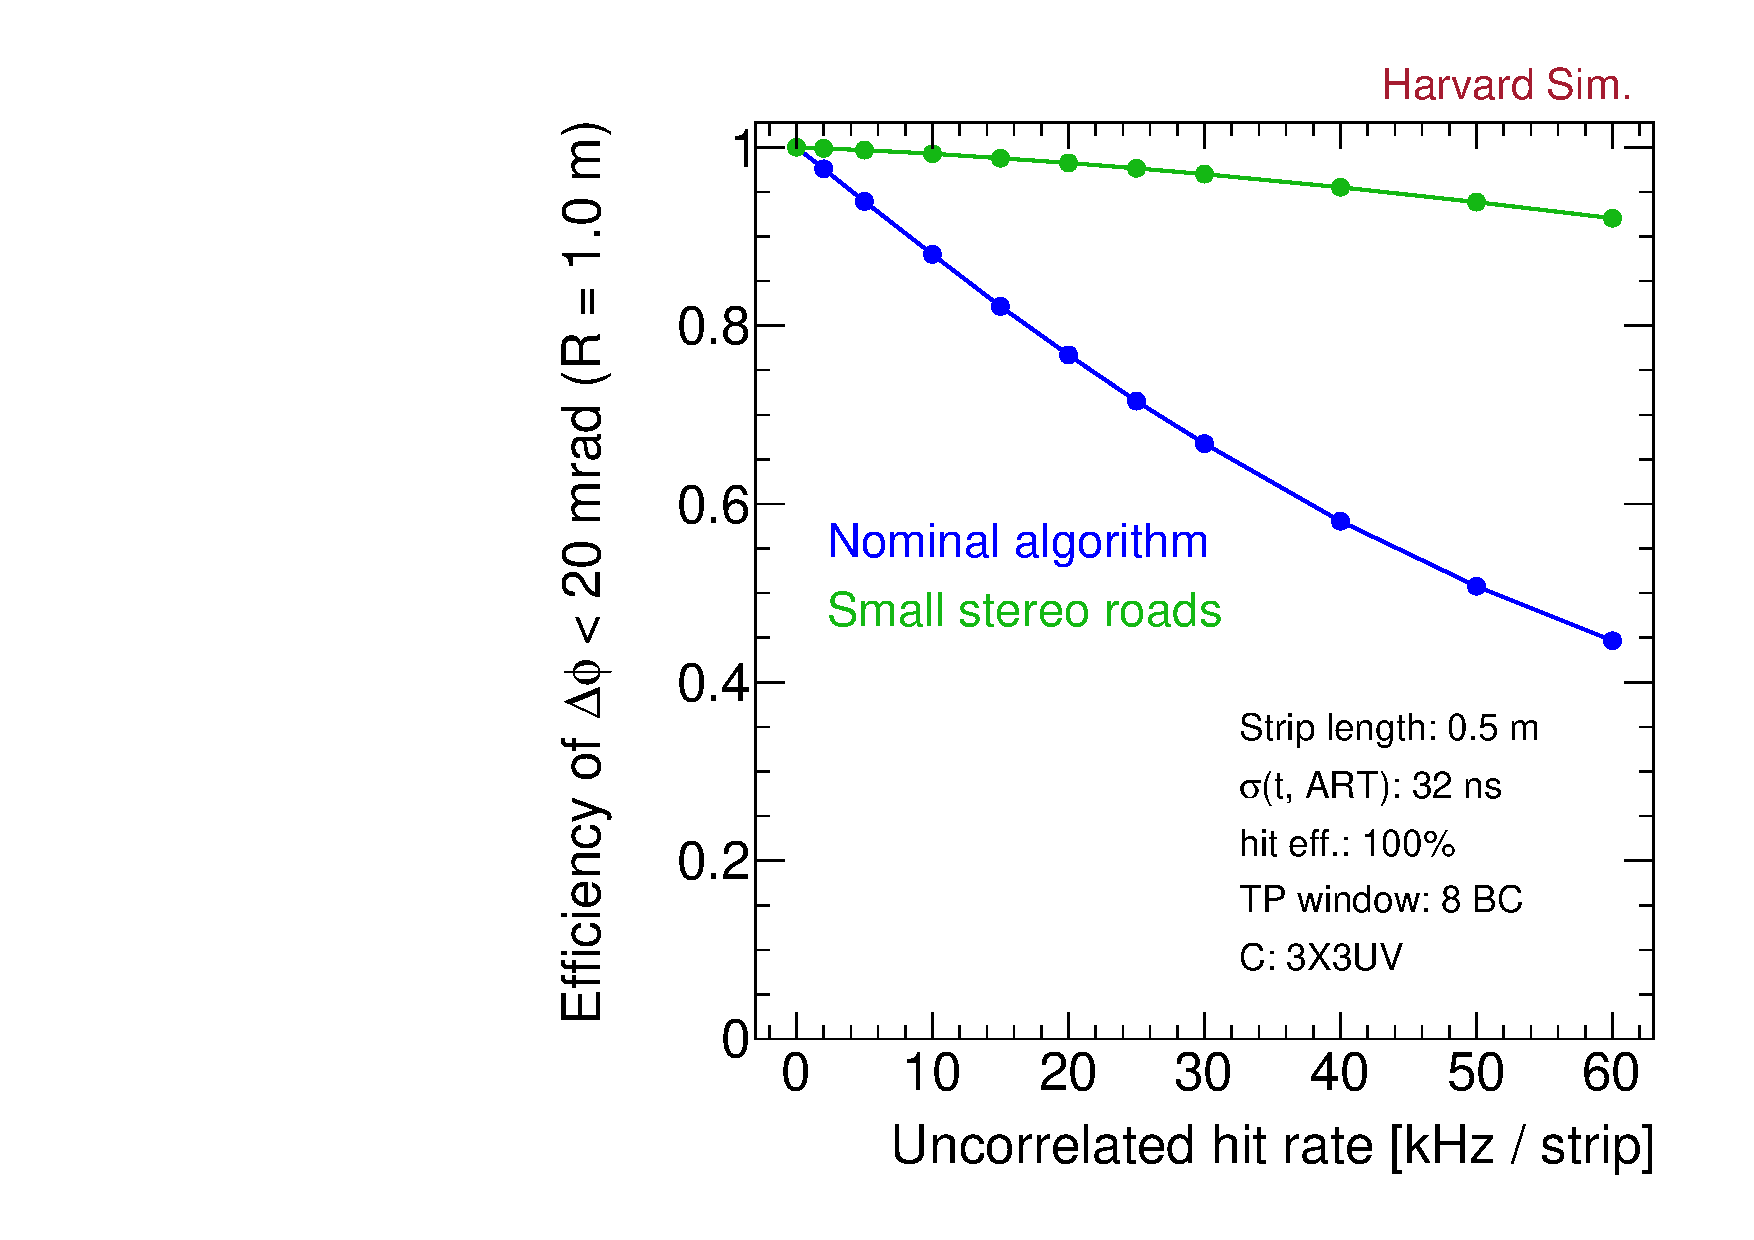
\includegraphics[width=0.48\textwidth]{figures/eff_phi_small_vs_rate.pdf}
    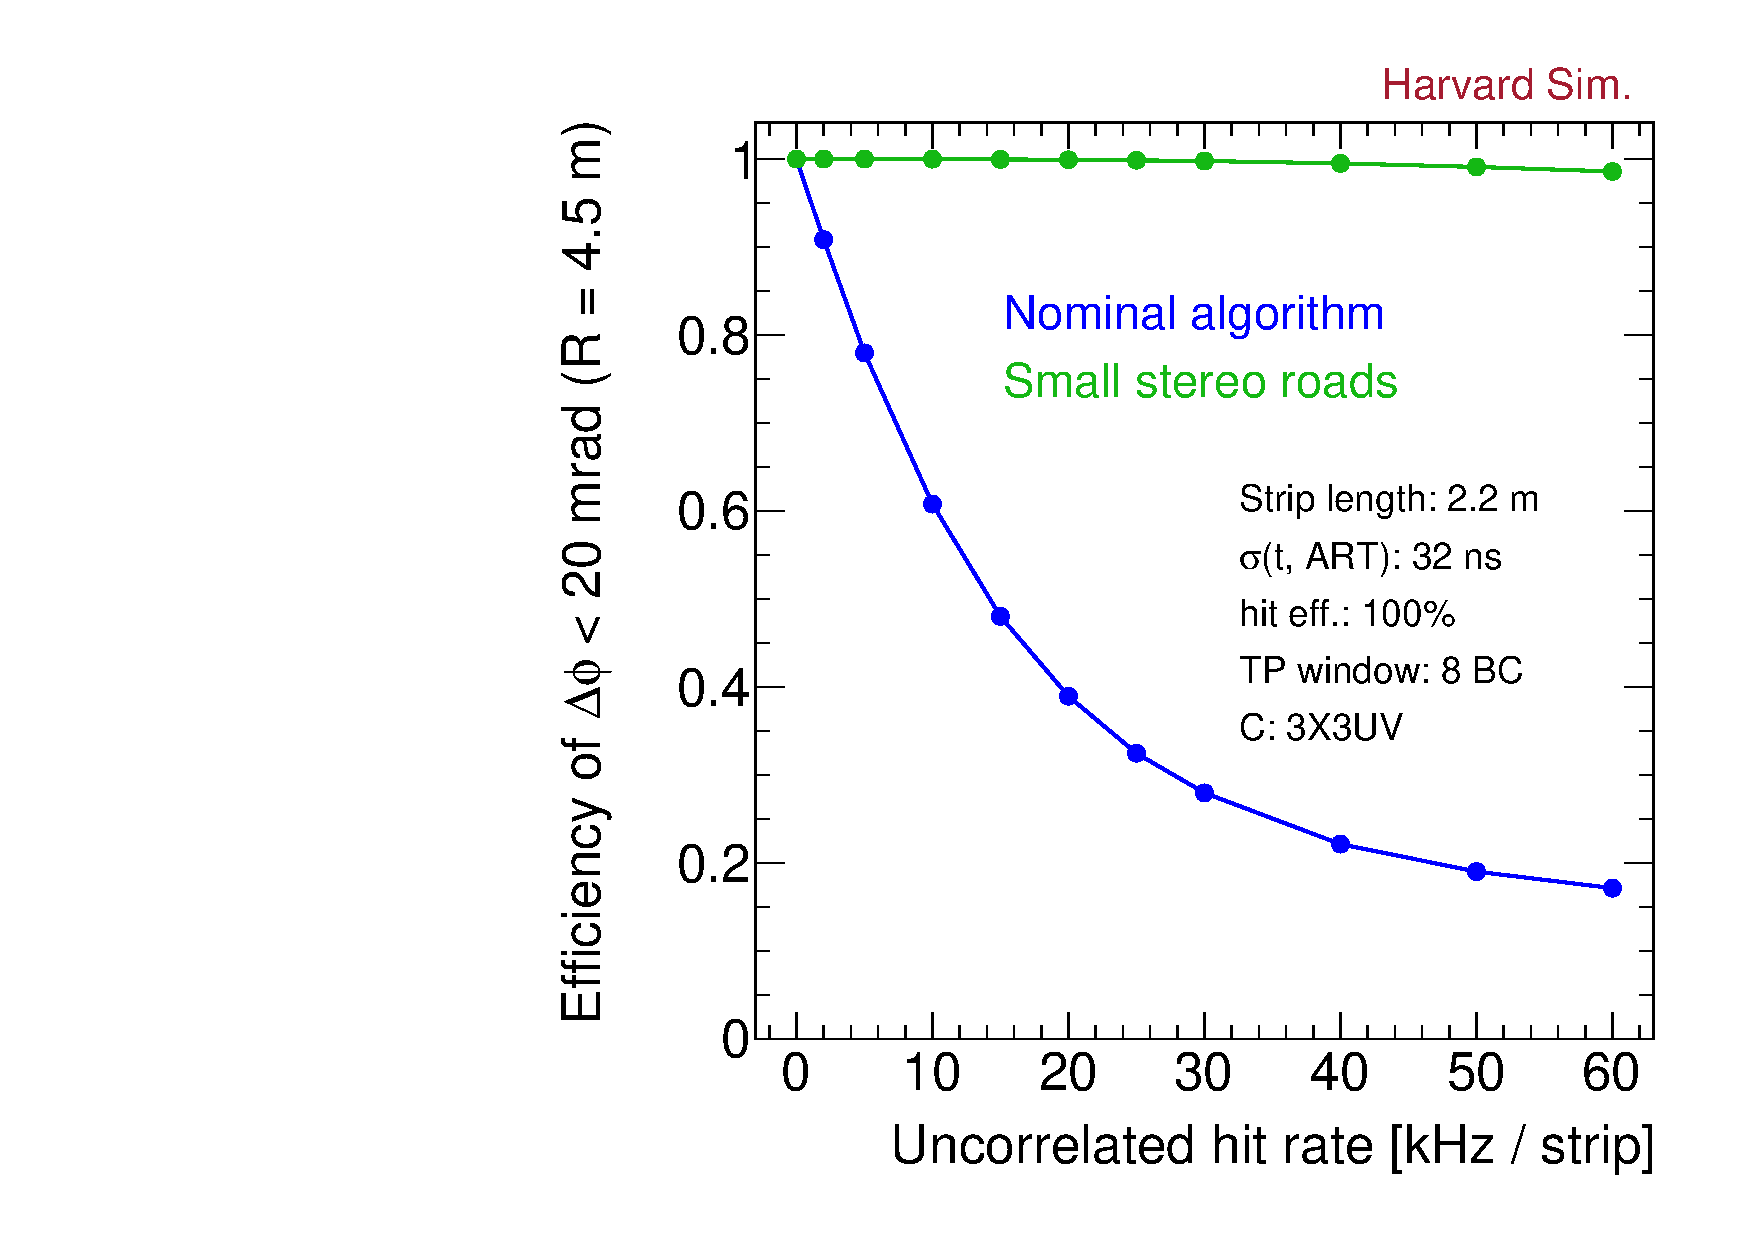
\includegraphics[width=0.48\textwidth]{figures/eff_phi_large_vs_rate.pdf}
  \end{center}
  \vspace{-10pt}
  \caption{Efficiency of $\phi_\text{reco.} - \phi_\text{truth} < 20 mrad$ for a small chamber (left) and large chamber (right). $\phi_\text{reco.}-\phi_\text{truth}$ is calculated as $\frac{y_\text{reco.} - y_\text{truth}}{R}$, where $R$ is the distance from the beamline. $R$ is taken to be 1m for the small chamber and 4.5m for the large chamber.}
  \label{fig:eff_vs_rate}
\end{figure}

